\documentclass{article}
\usepackage{relsize}
\usepackage{tikz}
\begin{document}


\pagestyle{empty}

  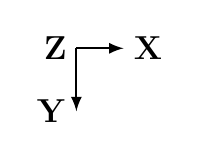
\begin{tikzpicture}[rotate=0]
    \draw[->, >=latex, thick] (0,0) -- (0,-0.8) node[left] {$\mathlarger{\mathlarger{\bf Y}}$};
    \draw[->, >=latex, thick] (0,0) -- (0.6,0) node[right] {$\mathlarger{\mathlarger{\bf X}}$};
    \draw (0,0) node[left] {$\mathlarger{\mathlarger{\bf Z}}$};
  \end{tikzpicture}

\end{document}



%%% Local Variables:
%%% mode: latex
%%% TeX-master: t
%%% End:
